\documentclass[border=1cm]{standalone}

\usepackage{tikz}

\usetikzlibrary{3d}

\begin{document}
    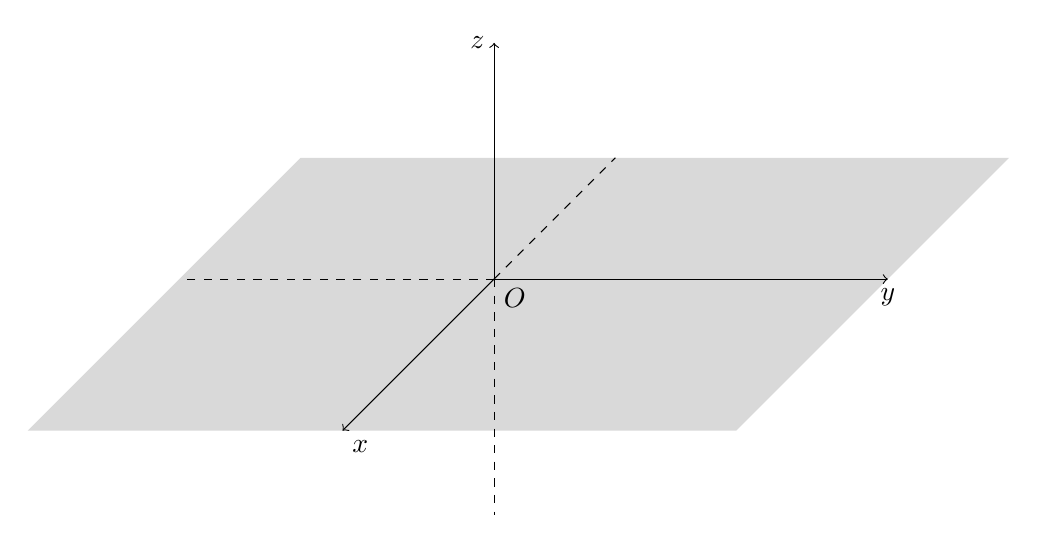
\begin{tikzpicture}
        \begin{scope}[canvas is xz plane at y=0]        
            \draw[draw=none, fill=gray!30] (-4,-4) rectangle (5,5);
        \end{scope}

        \draw[dashed] (0,0)--(-4,0);
        \draw[dashed] (0,0)--(0,-3);
        \draw[dashed] (0,0)--(0,0,-4);
        \draw[->] (0,0)--(5,0)node[below]{$y$};
        \draw[->] (0,0)--(0,3)node[left]{$z$};
        \draw[->] (0,0)--(0,0,5)node[below right]{$x$};
        \node at (0,0) [below right]{$O$};
    \end{tikzpicture}
\end{document}